
\textbf{Ingredients} Ingredients are plants or other elements useful for potion-making.

\begin{tabular}{m{2cm}m{3cm}m{10cm} } \hline
	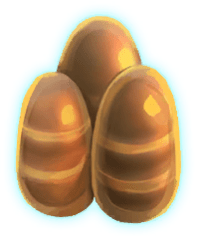
\includegraphics[width=2cm]{../Pictures/Gameplay/Items/Consumables/Ingredients/Ashwinder_eggs_picture.png} & \textbf{Ashwinder Egg} & Ashwinder eggs are the eggs of the Ashwinder , a magical serpent  which is born from the embers of an unattended magical fire. \\ \hline
	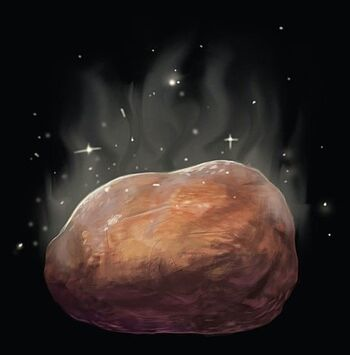
\includegraphics[width=2cm]{../Pictures/Gameplay/Items/Consumables/Ingredients/Bezoar_picture.png} & \textbf{Bezoar} & A bezoar is a stone-like mass taken from the stomach of a goat, that acts as an antitode to most potions \\ \hline
	
\includegraphics[width=2cm]{../Pictures/Gameplay/Items/Consumables/Ingredients/Bitter_root_picture.png} & \textbf{Bitter Root} & Bitter root (alternatively spelled bitterroot) is a plant that can be used as a potion ingredient. \\ \hline
	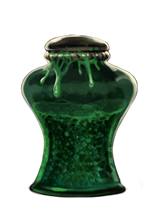
\includegraphics[width=2cm]{../Pictures/Gameplay/Items/Consumables/Ingredients/Flobberworm_mucus_picture.png} & \textbf{Flobberworm Mucus} & Flobberworm mucus, alternatively spelled Flobberworm mucous or Flobber Mucus for short, is the slimy green mucus exuded from the Flobberoworm, often used to thicken potions. \\ \hline
	
\includegraphics[width=2cm]{../Pictures/Gameplay/Items/Consumables/Ingredients/Granian_hair_picture.png} & \textbf{Granian Hair} & Granian hair is hair taken from a Granian Winged horse, which can be used as a potion ingredient. \\ \hline
	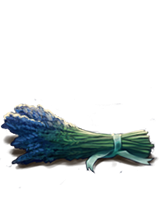
\includegraphics[width=2cm]{../Pictures/Gameplay/Items/Consumables/Ingredients/Lavender_picture.png} & \textbf{Lavender} & Lavender is a flower noted for its "beautiful colour" and "calming fragrance. It can be used as an ingredient in a variety of potions. \\ \hline
	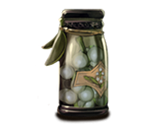
\includegraphics[width=2cm]{../Pictures/Gameplay/Items/Consumables/Ingredients/Mistletoe_berries_picture.png} & \textbf{Mistletoe Berries} & The berry of the mistletoe is small, white, and waxy. It is used as an ingredient in potion. \\ \hline
	
\includegraphics[width=2cm]{../Pictures/Gameplay/Items/Consumables/Ingredients/Murtlap_tentacle_picture.png} & \textbf{Murtlap Tentacle} & A Murtlap tentacle is a rare potion ingredient that can be obtained from the growth on the back of a Murtlap. \\ \hline
	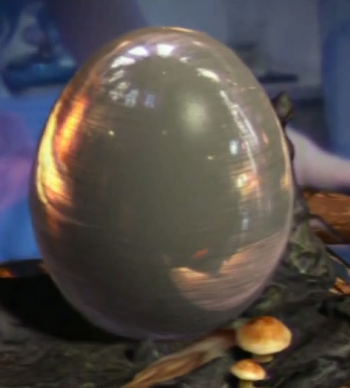
\includegraphics[width=2cm]{../Pictures/Gameplay/Items/Consumables/Ingredients/Occamy_egg_picture.png} & \textbf{Occamy Eggshell} & The egg of the Occamy has a shell made of pure silver, which accounts for why it is so much sought after. \\ \hline
	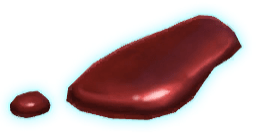
\includegraphics[width=2cm]{../Pictures/Gameplay/Items/Consumables/Ingredients/Reem_blood_picture.png} & \textbf{Re'em Blood} & Re'em blood gives the drinker immense strength for a short time. This in turn makes Re'em blood a highly desired substance, and a useful potion ingredient. \\ \hline
	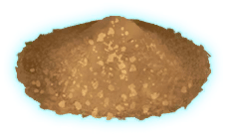
\includegraphics[width=2cm]{../Pictures/Gameplay/Items/Consumables/Ingredients/Rue_picture.png} & \textbf{Rue} & Rue, also known as common rue, is a kind of evergreen shrubs with a distinctive bitter taste. \\ \hline
	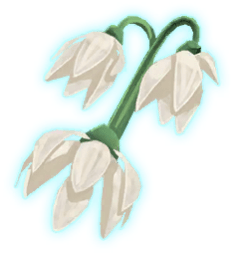
\includegraphics[width=2cm]{../Pictures/Gameplay/Items/Consumables/Ingredients/Snowdrop_picture.png} & \textbf{Snowdrop} & This plant is very well known for its stimulant properties. \\ \hline
\end{tabular}

\clearpage

\begin{tabular}{m{2cm}m{3cm}m{10cm} } \hline
	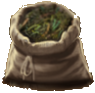
\includegraphics[width=2cm]{../Pictures/Gameplay/Items/Consumables/Ingredients/Standard_ingredient_picture.png} & \textbf{Standard Ingredient} & The Standard Ingredient is a herb, or mixture of dried herbs, with many magical applications and properties that is used as an ingredient in potion-making.  \\ \hline
	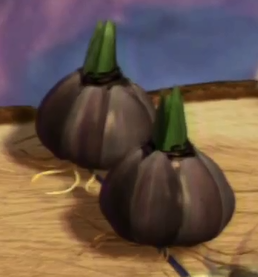
\includegraphics[width=2cm]{../Pictures/Gameplay/Items/Consumables/Ingredients/Squill_bulbs_picture.png} & \textbf{Squill Bulbs} & The bulb of the squill is a structure that functions as an organ for food storage while the plant is dormant. Squill bulbs have potion-making properties and are best harvested just after the plants blossoms. \\ \hline
	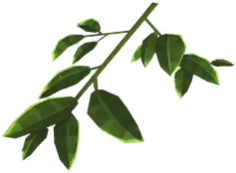
\includegraphics[width=2cm]{../Pictures/Gameplay/Items/Consumables/Ingredients/Tincture_of_thyme_picture.png} & \textbf{Tincture of Thyme} & Thyme is a common herb with culinary and medicinal uses, making it a good candidate for potion-making. \\ \hline
	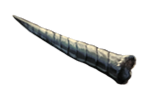
\includegraphics[width=2cm]{../Pictures/Gameplay/Items/Consumables/Ingredients/Unicorn_horn_picture.png} & \textbf{Unicorn Horn} & The horn of a unicorn had magical properties that made it a useful ingredient in potions. \\ \hline
	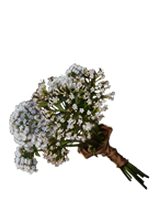
\includegraphics[width=2cm]{../Pictures/Gameplay/Items/Consumables/Ingredients/Valerian_picture.png} & \textbf{Valerian Sprigs} & Valerian is a plant with magical and calming properties. \\ \hline
\end{tabular}

\clearpage